\documentclass{article}

\usepackage{fancyhdr}
\usepackage{extramarks}
\usepackage{amsmath}
\usepackage{amsthm}
\usepackage{amsfonts}
\usepackage{tikz}
\usepackage[plain]{algorithm}
\usepackage{algpseudocode}
\usepackage{url}
\usepackage{listings}
\usepackage{xcolor}
\usepackage{hyperref}
\usepackage{graphicx}
\usepackage{placeins}
\usepackage{float}
\usepackage[utf8]{inputenc}
\usepackage{booktabs}
\usepackage{fontawesome5}

\graphicspath{{images/}}

% Define custom colors
\definecolor{codegreen}{rgb}{0,0.6,0}
\definecolor{codegray}{rgb}{0.5,0.5,0.5}
\definecolor{codepurple}{rgb}{0.58,0,0.82}
\definecolor{backcolour}{rgb}{0.95,0.95,0.92}

% Setup the style
\lstdefinestyle{mystyle}{
    backgroundcolor=\color{backcolour},
    commentstyle=\color{codegreen},
    keywordstyle=\color{magenta},
    numberstyle=\tiny\color{codegray},
    stringstyle=\color{codepurple},
    basicstyle=\ttfamily\footnotesize,
    breakatwhitespace=false,
    breaklines=true,
    captionpos=b,
    keepspaces=true,
    numbers=left,
    numbersep=5pt,
    showspaces=false,
    showstringspaces=false,
    showtabs=false,
    tabsize=2
}
\lstset{style=mystyle}

\usetikzlibrary{automata,positioning}

%
% Basic Document Settings
%
\topmargin=-0.45in
\evensidemargin=0in
\oddsidemargin=0in
\textwidth=6.5in
\textheight=9.0in
\headsep=0.25in

\linespread{1.1}

\pagestyle{fancy}
\lhead{\hmwkAuthorName}
\chead{\hmwkClass\ (\hmwkClassInstructor\ \hmwkClassTime): \hmwkTitle}
\rhead{\firstxmark}
\lfoot{\lastxmark}
\cfoot{\thepage}

\renewcommand\headrulewidth{0.4pt}
\renewcommand\footrulewidth{0.4pt}

\setlength\parindent{0pt}

%
% Create Problem Sections
%
\newcommand{\enterProblemHeader}[1]{
    \nobreak\extramarks{}{Problem \arabic{#1} continued on next page\ldots}\nobreak{}
    \nobreak\extramarks{Problem \arabic{#1} (continued)}{Problem \arabic{#1} continued on next page\ldots}\nobreak{}
}

\newcommand{\exitProblemHeader}[1]{
    \nobreak\extramarks{Problem \arabic{#1} (continued)}{Problem \arabic{#1} continued on next page\ldots}\nobreak{}
    \stepcounter{#1}
    \nobreak\extramarks{Problem \arabic{#1}}{}\nobreak{}
}

\setcounter{secnumdepth}{0}
\newcounter{partCounter}
\newcounter{homeworkProblemCounter}
\setcounter{homeworkProblemCounter}{1}
\nobreak\extramarks{Problem \arabic{homeworkProblemCounter}}{}\nobreak{}

%
% Homework Problem Environment
%
\newenvironment{homeworkProblem}[1][-1]{
    \ifnum#1>0
        \setcounter{homeworkProblemCounter}{#1}
    \fi
    \section{Question \arabic{homeworkProblemCounter}}
    \setcounter{partCounter}{1}
    \enterProblemHeader{homeworkProblemCounter}
}{
    \exitProblemHeader{homeworkProblemCounter}
}

%
% Homework Details
%
\newcommand{\hmwkTitle}{Homework\ \#5}
\newcommand{\hmwkDueDate}{21st April 2026}
\newcommand{\hmwkClass}{IEOR 4578}
\newcommand{\hmwkClassTime}{}
\newcommand{\hmwkClassInstructor}{}
\newcommand{\hmwkAuthorName}{\textbf{Luca Barattini - UNI: LB3656}}

% GitHub repository link
\newcommand{\hmwkNbURL}{https://github.com/lucabarattini/IEOR-4578/blob/main/HW5/Basis_Notebook.ipynb}

%
% Title Page
%
\hypersetup{
    colorlinks=true,
    linkcolor=blue,
    filecolor=magenta,
    urlcolor=blue,
}

\title{
    \vspace{2in}
    \textmd{\textbf{\hmwkClass:\ \hmwkTitle}}\\
    \normalsize\vspace{0.1in}\small{Due\ on\ \hmwkDueDate}\\
    \vspace{0.1in}\large{\textit{\hmwkClassInstructor\ \hmwkClassTime}}\\
    \vspace{0.25in}
    \large{
        \textbf{Code Repository:} \\
        \vspace{0.1in}
        \href{\hmwkNbURL}{\faGithub \ Basis Notebook}
    }
    \vspace{3in}
}

\author{\hmwkAuthorName}
\date{}

\renewcommand{\part}[1]{\textbf{\large Part \Alph{partCounter}}\stepcounter{partCounter}\\}

%
% Various Helper Commands
%
\newcommand{\solution}{\textbf{\large Solution}}

\begin{document}

\maketitle
\pagebreak

% ==========================================
% QUESTION 1
% ==========================================
\begin{homeworkProblem}

\textbf{Run the Basis functions related code shared in the ``Basis.py'' file. [Points 50]}
\begin{itemize}
    \item Explain Piecewise constant fit.
    \item Explain Piecewise linear fit.
    \item Explain Continuous Piecewise Linear.
    \item Explain Continuous cubic spline fit.
\end{itemize}

\subsection*{Setup}

I generate $50$ samples on $x \in [-1, 7]$ from $y = \cos(x)$, then add Gaussian noise with $\sigma = 0.5$ to mimic real-world measurement error. The result is a set of noisy points scattered around a smooth cosine curve.\\
\\
\textbf{What is a knot?}\\
\\
A \textbf{knot} is a point along the x-axis where I allow the fitted curve to change behavior. Think of it as a fence post that divides the data into separate regions. Inside each region the curve can have its own shape, and at each knot the curve can either jump (discontinuous fit) or bend smoothly (continuous fit), depending on the method.\\
\\
For this question I place two interior knots that split the cosine domain into three roughly equal-width regions:
$$x_{\min} = -1, \qquad x_{\text{knot}_1} = 1.5, \qquad x_{\text{knot}_2} = 4.5, \qquad x_{\max} = 7.$$

\begin{figure}[H]
     \centering
     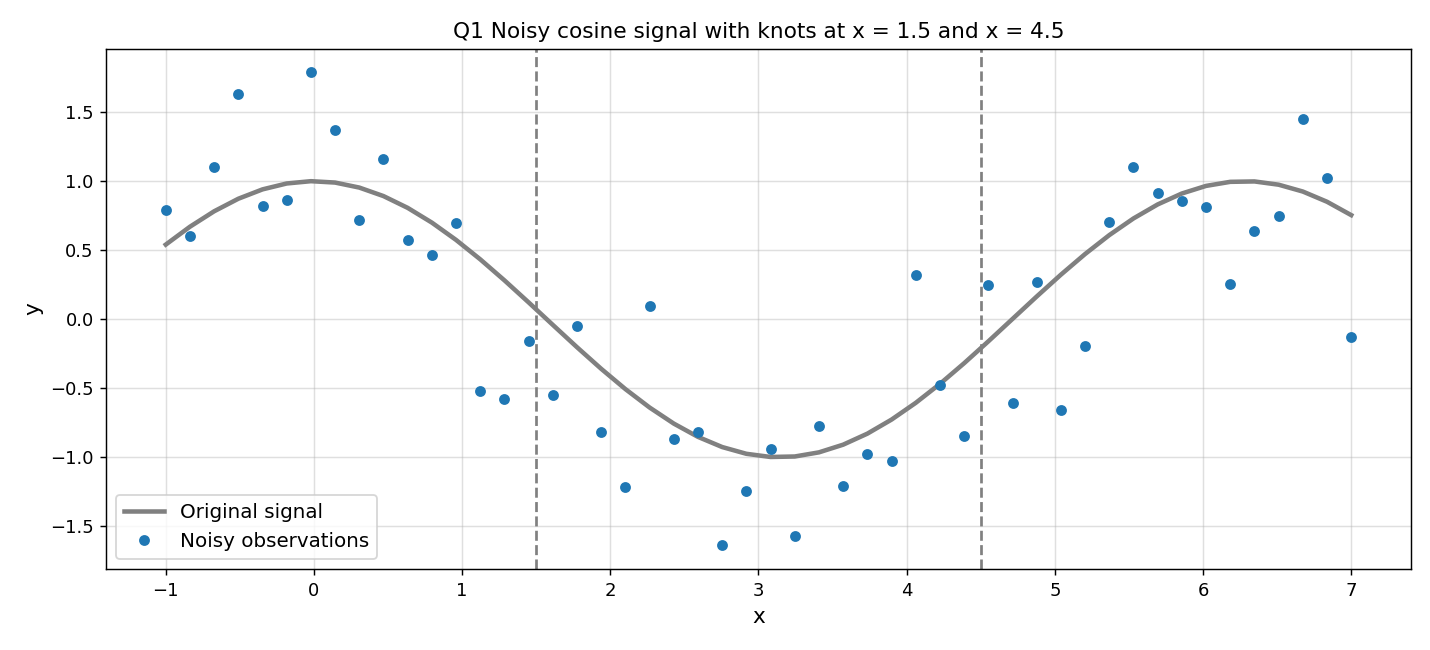
\includegraphics[width=\textwidth]{Q1_signal.png}
     \caption{Q1 raw data: noisy cosine signal (blue dots) around the true signal (grey curve). Dashed grey lines mark the two knots at $x = 1.5$ and $x = 4.5$.}
     \label{fig:q1_signal}
\end{figure}

\hrulefill

\subsection*{Part a) Piecewise Constant Fit}

The simplest possible fit: inside each region, replace the data by the average value of $y$ in that region. Mathematically:
$$\hat{y}(x) \;=\; \bar{y}_{\text{region}(x)}.$$

The fitted function looks like a staircase, with one horizontal step per region and two jumps at the knots. It captures the average level inside each piece, but ignores any slope or shape.

\begin{lstlisting}[language=Python, title={Python Console Output: Regional Means}]
Region 1 mean:  0.7212
Region 2 mean: -0.6710
Region 3 mean:  0.6465
\end{lstlisting}

\textbf{Conclusion:}\\
\\
Each regional mean correctly reflects whether that piece of the cosine wave is mostly above or below zero. Region~1 ($x \in [-1, 1.5]$) covers the first peak of the cosine (near $x = 0$, where $\cos = +1$), so its mean is positive ($+0.72$). Region~2 ($x \in [1.5, 4.5]$) brackets the trough near $x = \pi \approx 3.14$ where $\cos = -1$, so its mean is negative ($-0.67$). Region~3 ($x \in [4.5, 7]$) climbs back toward the next peak near $x = 2\pi$, so its mean is again positive ($+0.65$). The staircase shape clearly misses the smooth oscillation between knots.

\begin{figure}[H]
     \centering
     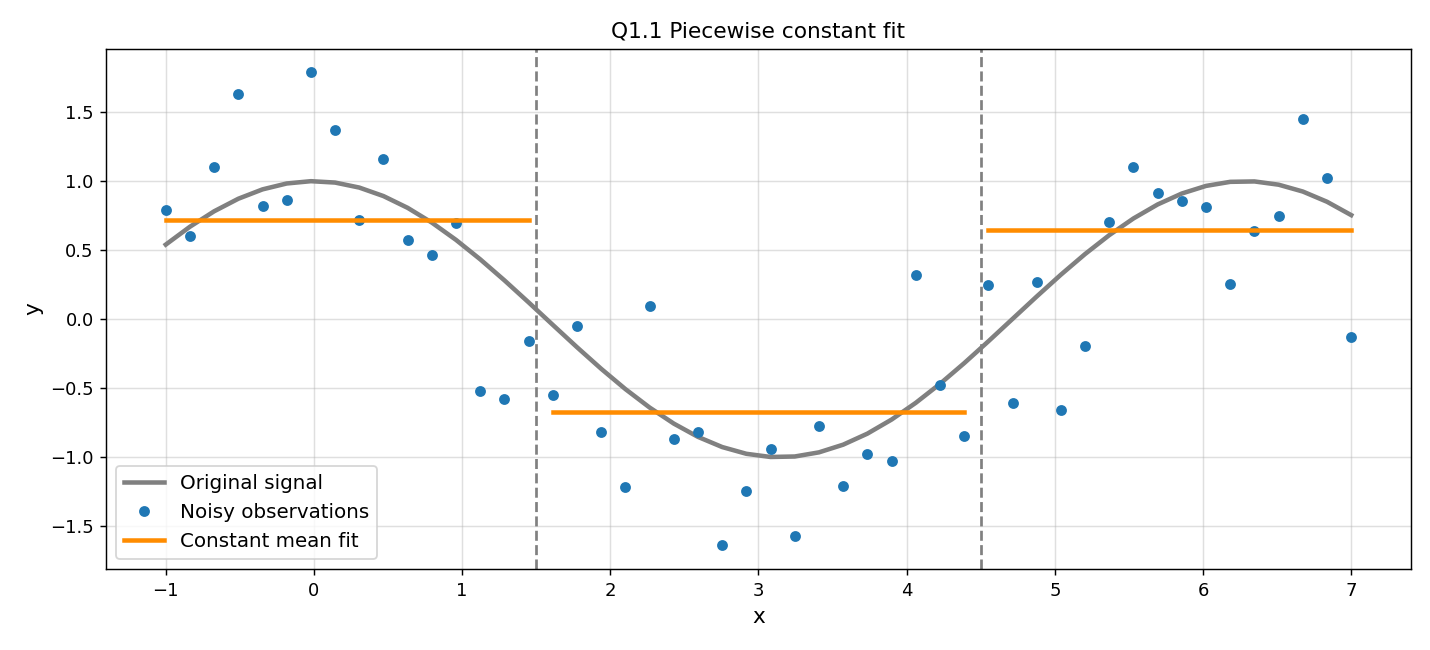
\includegraphics[width=\textwidth]{Q1_piecewise_constant.png}
     \caption{Q1.1 Piecewise constant fit. Each orange segment is the mean of the cosine inside one region.}
     \label{fig:q1_pc}
\end{figure}

\subsection*{Part b) Piecewise Linear Fit}

Now fit an independent straight line $y = \alpha_r + \beta_r x$ inside each region $r$, using the standard ordinary-least-squares (OLS) formulas. The notebook uses a slightly compact form,
$$\hat{\alpha}_r \;=\; \bar{y}_r, \qquad \hat{\beta}_r \;=\; \frac{(y_r - \bar{y}_r) \cdot x_r}{\sum x_r^2},$$
which is just the textbook OLS solution rewritten by mean-centering $y$ first.\\
\\
\textbf{What the formula says, in plain English:}
\begin{itemize}
    \item $\hat{\alpha}_r = \bar{y}_r$: the intercept of the line in region $r$ is the average of $y$ in that region.
    \item $\hat{\beta}_r = \dfrac{(y_r - \bar{y}_r) \cdot x_r}{\sum x_r^2}$: the slope is computed by taking how far each $y$ is from its regional mean, weighting by the corresponding $x$, summing, and dividing by the total ``size'' of $x$. It measures the linear trend of the data within the region.
\end{itemize}
This produces three independent straight lines, one per region. The lines do not have to meet at the knots, so the fit is still discontinuous there.

\begin{lstlisting}[language=Python, title={Python Console Output: Regional Slopes}]
Region 1 slope: -0.1719
Region 2 slope: -0.0083
Region 3 slope:  0.0068
\end{lstlisting}

\textbf{Conclusion:}\\
\\
All three slopes are very small. The reason is that each region spans roughly half a full cosine cycle (cosine has period $2\pi \approx 6.28$, and my regions are about $2.5$ to $3$ units wide, so each one covers about a half-period). Inside a half-period the cosine goes up and then back down (or vice versa), and a single straight line trying to summarize that wave-shaped motion ends up nearly horizontal because the rising and falling parts cancel out. The fit is more flexible than the piecewise constant version because it now allows a tilt in each piece, but it still has visible jumps at the knots.

\begin{figure}[H]
     \centering
     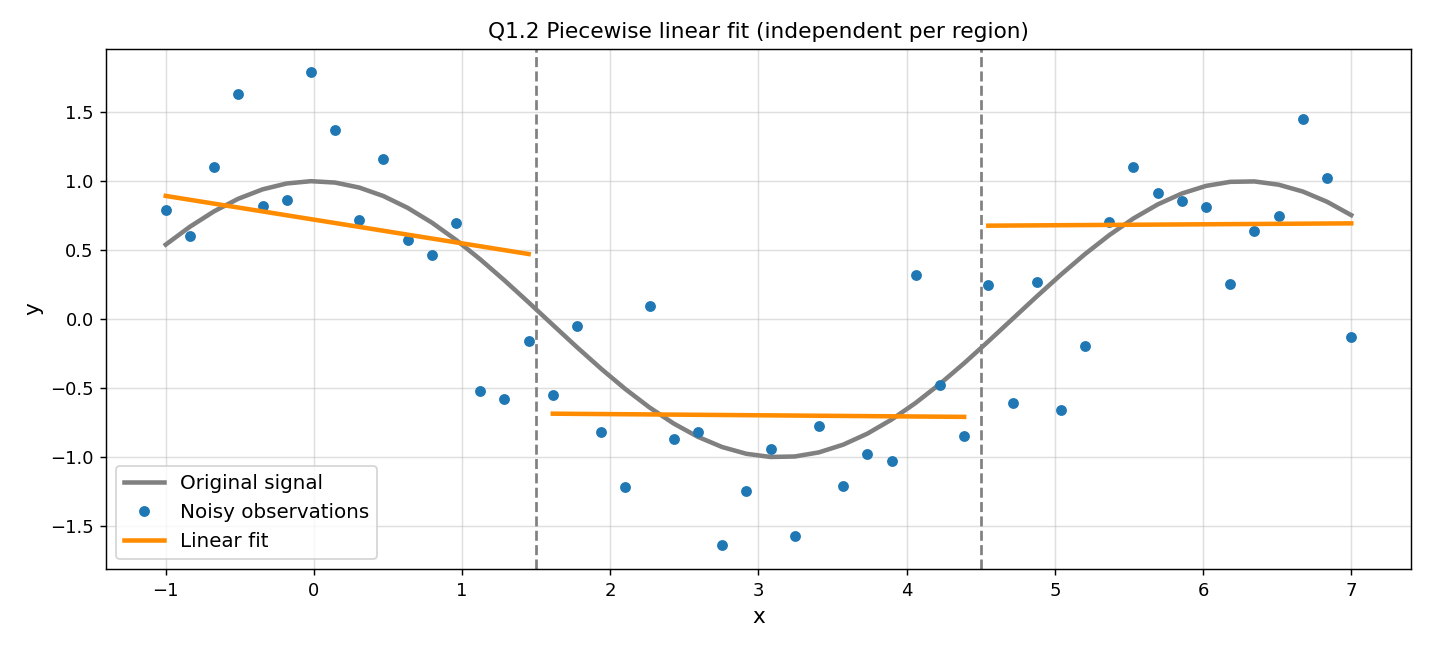
\includegraphics[width=\textwidth]{Q1_piecewise_linear.png}
     \caption{Q1.2 Piecewise linear fit. Three independent OLS lines, one per region. Visible jumps at the knots.}
     \label{fig:q1_pl}
\end{figure}

\subsection*{Part c) Continuous Piecewise Linear}

To remove the jumps at the knots, I fit all three pieces \emph{jointly} using ordinary least squares on four basis functions:
$$\hat{y}(x) \;=\; \beta_0 + \beta_1 x + \beta_2 (x - x_{\text{knot}_1})_+ + \beta_3 (x - x_{\text{knot}_2})_+,$$
where $(\cdot)_+ = \max(\cdot, 0)$. The two truncated linear terms act as ``hinges'' at the knots: they let the slope change there while keeping the function value continuous (no jumps).

\begin{lstlisting}[language=Python, title={Python Console Output: Beta Coefficients}]
Beta coefficients (h1, h2, h3, h4): [ 0.7680  -0.8663  0.8449  0.7402 ]
\end{lstlisting}

\textbf{Conclusion:}\\
\\
The hinge coefficients add up cumulatively to give the slope inside each region:
\begin{itemize}
    \item Region 1 ($x < 1.5$): slope $= \beta_1 = -0.87$ (steep decline).
    \item Region 2 ($1.5 \leq x < 4.5$): slope $= \beta_1 + \beta_2 = -0.02$ (almost flat through the trough).
    \item Region 3 ($x \geq 4.5$): slope $= \beta_1 + \beta_2 + \beta_3 = +0.72$ (climbing back up).
\end{itemize}
The fit is continuous at both knots and tracks the cosine direction in each region, but cannot follow the curvature inside the trough.

\begin{figure}[H]
     \centering
     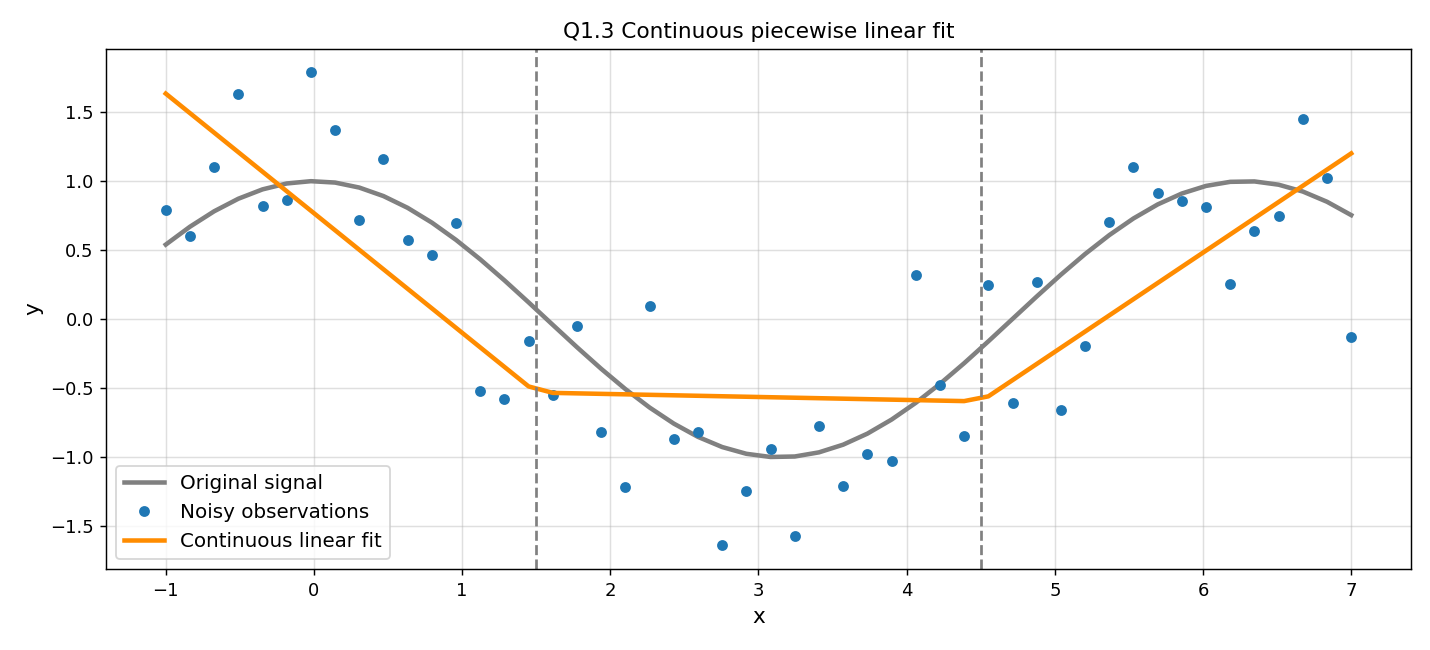
\includegraphics[width=\textwidth]{Q1_continuous_linear.png}
     \caption{Q1.3 Continuous piecewise linear fit. One curve made of three line segments joined at the knots.}
     \label{fig:q1_cpl}
\end{figure}

\subsection*{Part d) Continuous Cubic Spline}

Same basis-expansion idea as Part~c, but now with cubic building blocks instead of straight lines:
$$\hat{y}(x) \;=\; \beta_0 + \beta_1 x + \beta_2 x^2 + \beta_3 x^3 + \beta_4 (x - x_{\text{knot}_1})_+^3 + \beta_5 (x - x_{\text{knot}_2})_+^3.$$

The first four bases ($1, x, x^2, x^3$) give a global cubic polynomial. The two truncated cubic bases $(x - x_k)_+^3$ are the cubic version of the hinges from Part~c: they are zero before the knot and then grow as a cubic afterwards. They let the curve change shape at each knot \emph{without} introducing a jump in value, slope, or curvature. The fit is therefore smooth in value, slope, and curvature across the knots.

\begin{lstlisting}[language=Python, title={Python Console Output: Beta Coefficients}]
Beta coefficients (h1..h6): [ 1.0862  -0.1743  -0.6845  0.1983  -0.1792  -0.2507 ]
\end{lstlisting}

\textbf{Conclusion:}\\
\\
This is the best of the four fits for the cosine signal. The underlying generating function $\cos(x)$ is itself smooth in value, slope, and curvature, so a smooth piecewise cubic matches the data structure perfectly. The fitted curve sits almost on top of the noiseless signal and bends gracefully through both knots.

\begin{figure}[H]
     \centering
     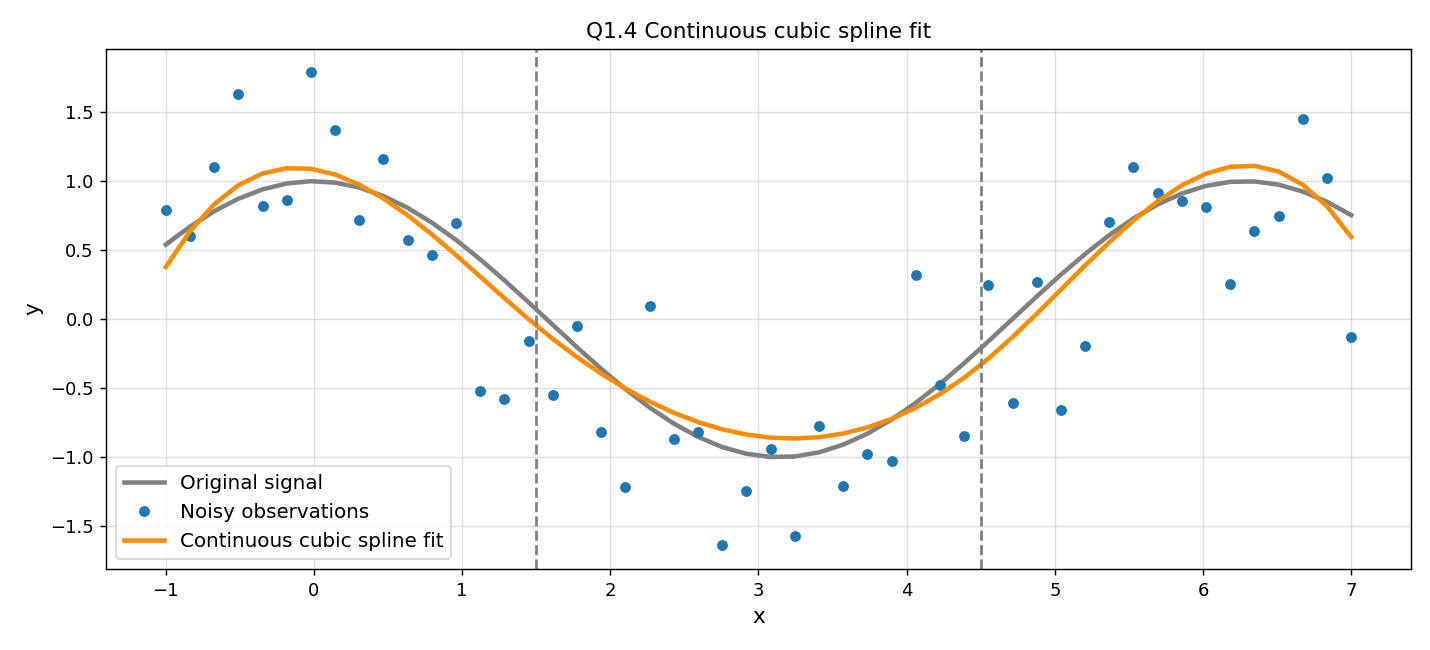
\includegraphics[width=\textwidth]{Q1_cubic_spline.png}
     \caption{Q1.4 Continuous cubic spline fit. The smoothest of the four fits, sitting nearly on top of the true cosine.}
     \label{fig:q1_cs}
\end{figure}

\end{homeworkProblem}
\hrule
\vspace{4mm}

% ==========================================
% QUESTION 2
% ==========================================
\begin{homeworkProblem}

\textbf{Run the Basis functions related code shared in the ``Basis.py'' file for the ``WholeFood.xlsx'' data. [Points 50]}
\begin{itemize}
    \item Explain Piecewise constant fit.
    \item Explain Piecewise linear fit.
    \item Explain Continuous Piecewise Linear.
    \item Explain Continuous cubic spline fit is not a good fit for this data.
\end{itemize}

\subsection*{Setup}

The dataset has $248$ weekly observations and a single column \texttt{Weekly Sales}. I index time by row number ($x = 0, 1, \ldots, 247$), so each $x$ value is simply ``which week''. I place two interior knots at the $1/3$ and $2/3$ marks of the timeline so that the three regions are roughly equal width:
$$x_{\min} = 0, \qquad x_{\text{knot}_1} = 82, \qquad x_{\text{knot}_2} = 165, \qquad x_{\max} = 247.$$

Unlike the cosine in Q1, here there is no underlying ``true signal'': the observed weekly sales \emph{are} the data.

\begin{figure}[H]
     \centering
     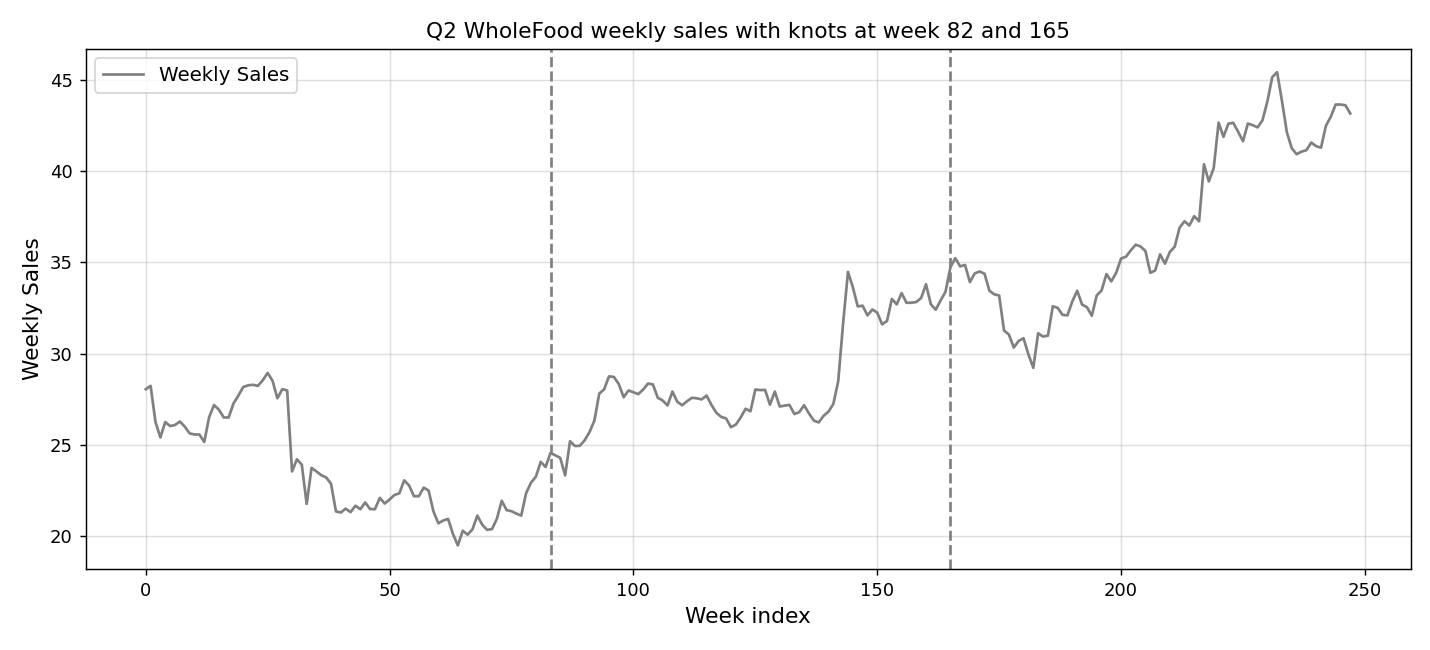
\includegraphics[width=\textwidth]{Q2_signal.png}
     \caption{Q2 raw data: WholeFood weekly sales over 248 weeks. Knots at week 82 and week 165 marked with dashed grey lines.}
     \label{fig:q2_signal}
\end{figure}

\hrulefill

\subsection*{Part a) Piecewise Constant Fit}

Same idea as Q1.a: inside each region, replace the data by the average of \texttt{Weekly Sales} in that region. The fitted function is a three-step staircase.

\begin{lstlisting}[language=Python, title={Python Console Output: Regional Means}]
Region 1 mean: 23.7733
Region 2 mean: 28.5679
Region 3 mean: 36.9540
\end{lstlisting}

\textbf{Conclusion:}\\
\\
The three means rise across time: $\approx 23.8$ in the early weeks, $\approx 28.6$ in the middle, $\approx 37.0$ in the late weeks. This already exposes the underlying upward drift in the series, but the staircase ignores any week-to-week trend inside each region.

\begin{figure}[H]
     \centering
     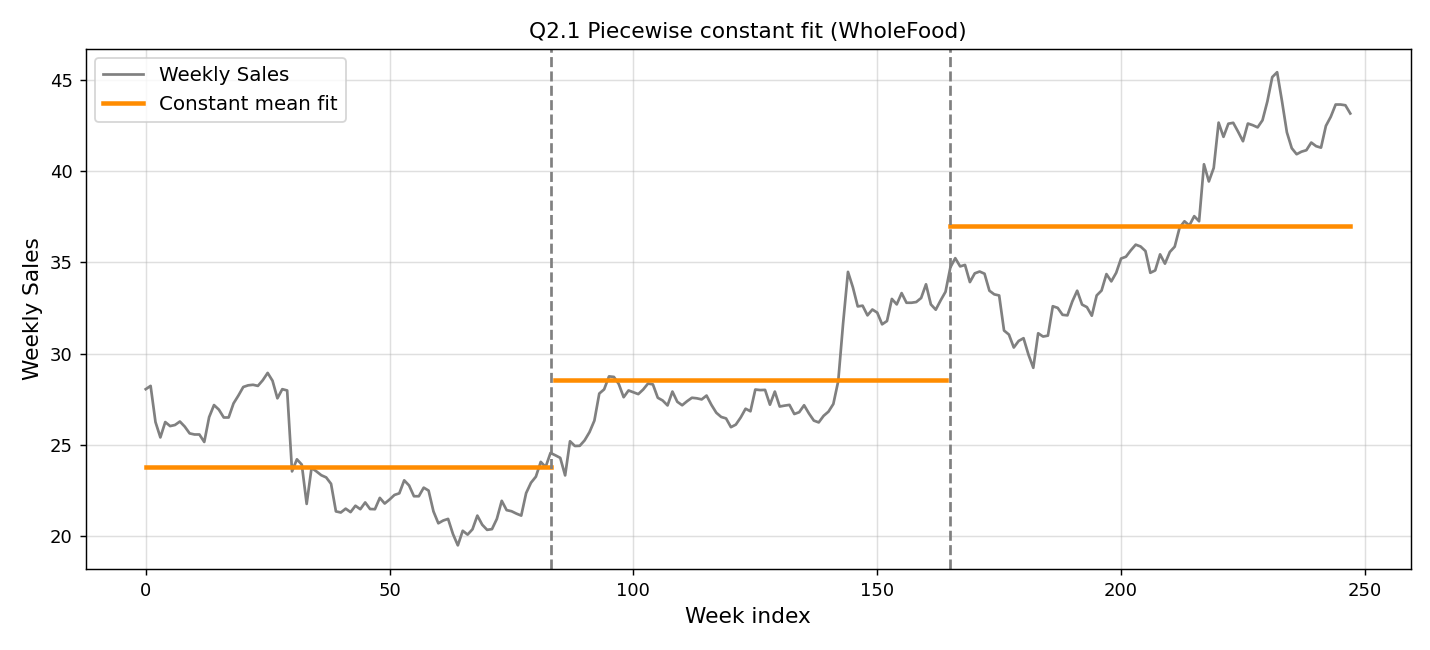
\includegraphics[width=\textwidth]{Q2_piecewise_constant.png}
     \caption{Q2.1 Piecewise constant fit. Three horizontal levels equal to the regional sales averages.}
     \label{fig:q2_pc}
\end{figure}

\subsection*{Part b) Piecewise Linear Fit}

Same independent-OLS-per-region method as Q1.b. Each region now gets its own straight line with its own intercept and slope, but the three lines are not forced to meet at the knots.

\begin{lstlisting}[language=Python, title={Python Console Output: Regional Slopes}]
Region 1 slope: -0.0216
Region 2 slope:  0.0031
Region 3 slope:  0.0022
\end{lstlisting}

\textbf{Conclusion:}\\
\\
Region~1 slopes very slightly downward, Regions~2 and 3 slope very slightly upward. The slopes themselves are tiny in absolute value because the regions are wide ($\approx 82$ weeks each) and the per-region average trend gets diluted by week-to-week noise. The fit is still discontinuous at the knots.

\begin{figure}[H]
     \centering
     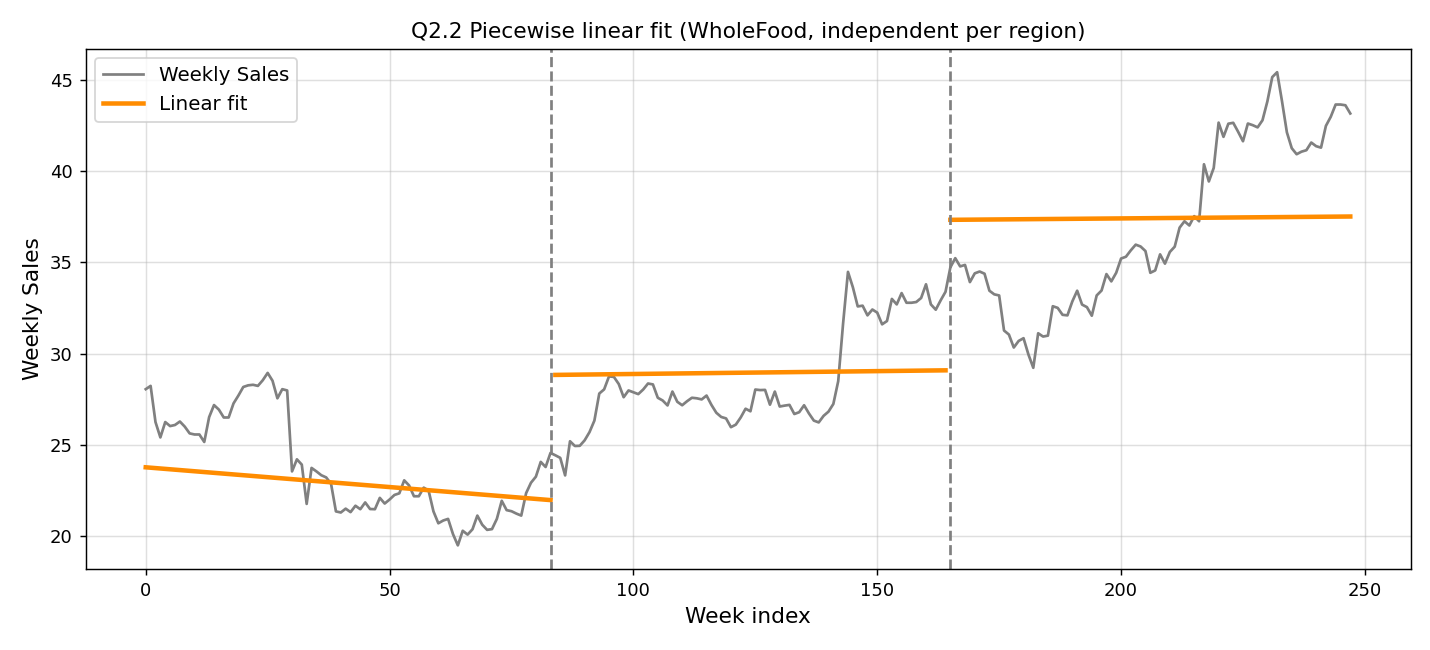
\includegraphics[width=\textwidth]{Q2_piecewise_linear.png}
     \caption{Q2.2 Piecewise linear fit. Three independent OLS lines, one per region.}
     \label{fig:q2_pl}
\end{figure}

\subsection*{Part c) Continuous Piecewise Linear}

Same truncated-linear basis expansion as Q1.c, with knots at week 82 and 165.

\begin{lstlisting}[language=Python, title={Python Console Output: Beta Coefficients}]
Beta coefficients (h1, h2, h3, h4): [ 25.9912  -0.0371  0.1468  0.0243 ]
\end{lstlisting}

\textbf{Conclusion:}\\
\\
The cumulative slopes across the three regions are $-0.04$, $+0.11$, and $+0.13$: a mild contraction in the early weeks, a clear shift to growth at week 82, and slightly faster growth after week 165. This is the most informative of the four fits for this series, capturing three growth regimes joined cleanly at the structural breaks.

\begin{figure}[H]
     \centering
     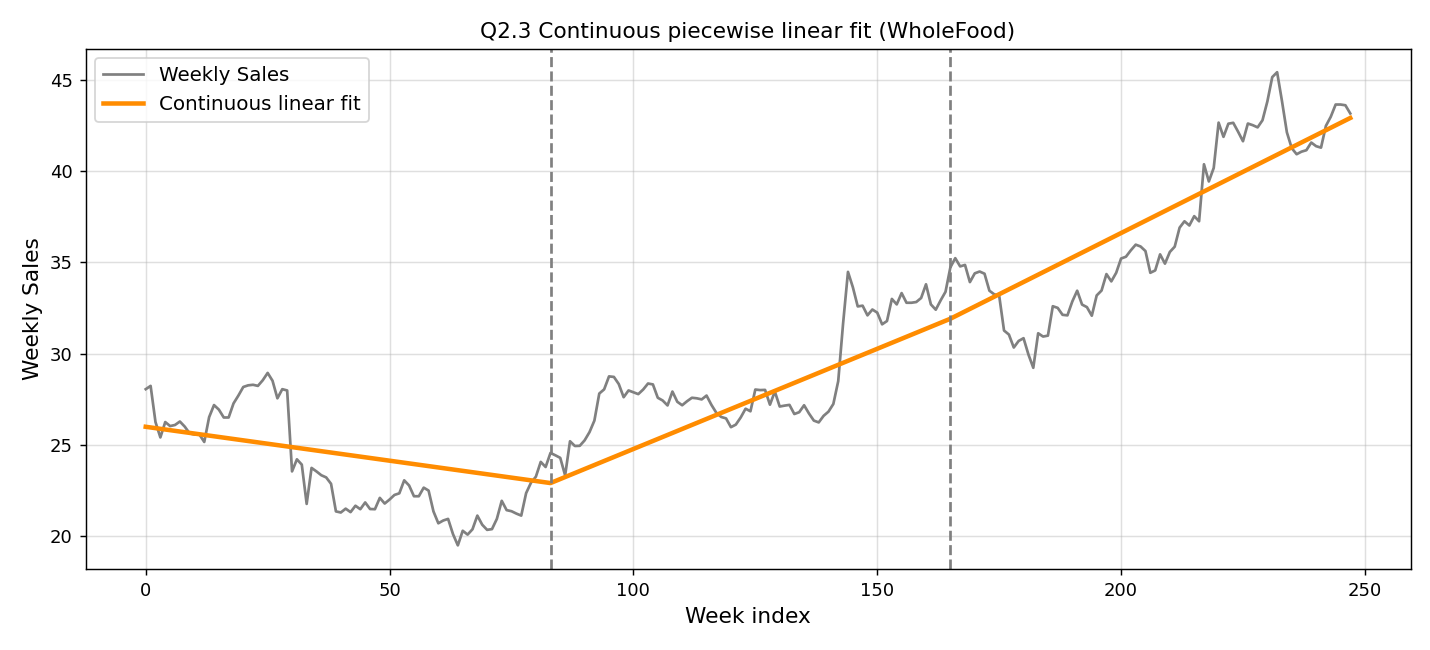
\includegraphics[width=\textwidth]{Q2_continuous_linear.png}
     \caption{Q2.3 Continuous piecewise linear fit. Three line segments joined at week 82 and week 165.}
     \label{fig:q2_cpl}
\end{figure}

\subsection*{Part d) Continuous Cubic Spline}

Same cubic-spline basis as Q1.d, applied to the WholeFood data. I include a diagnostic on the conditioning of the basis matrix to motivate the discussion below.

\begin{lstlisting}[title={Python Console Output: Diagnostics and Coefficients}, basicstyle=\ttfamily]
Condition number of H'H : 1.04e+15
Residual sum of squares : 990.98
Beta coefficients       : [ 2.9168e+01  -2.7305e-01  3.3990e-03  -1.0000e-05  5.0000e-06  2.4000e-05 ]
\end{lstlisting}

\subsubsection*{Why the Cubic Spline is Not a Good Fit Here}

Two issues, both visible in Figure~\ref{fig:q2_cs}:\\

\textbf{1. The data have no local cubic structure.}\\
Inside each region the WholeFood series is essentially linear with sharp ``kinks'' at the knots (changes in growth regime). A cubic basis adds curvature that the data simply do not contain, so the fit just bends gently across the whole series and smooths the kinks away. The continuous piecewise linear fit in Part~c already captures the genuine structure (three slopes joined at the knots) without that unnecessary curvature.\\

\textbf{2. The basis is numerically unstable.}\\
With $x \in [0, 247]$, the basis columns $x$, $x^2$, $x^3$ span seven orders of magnitude (since $247 \approx 10^{2.4}$, $247^2 \approx 10^{4.8}$, $247^3 \approx 10^{7.2}$).\\
\\
This makes the matrix $H^\top H$ \emph{nearly singular}. Its condition number is $\kappa \approx 10^{15}$, which means small numerical errors get amplified by a factor of $10^{15}$ when solving the normal equations. As a result, the cubic coefficients ($10^{-5}$ to $10^{-6}$) are essentially noise: they are not meaningfully identified.\\
\\
The same basis works fine on the cosine example because there $x$ stays inside $[-1, 7]$, where $x^3$ is at most $\sim 343$, and the conditioning is harmless.\\

\textbf{Conclusion:}\\
\\
For the WholeFood series, the continuous piecewise linear fit from Part~c is the appropriate choice. The cubic spline is both mathematically inappropriate (the data are piecewise linear, not piecewise cubic) and numerically unstable (the design matrix is nearly singular).

\begin{figure}[H]
     \centering
     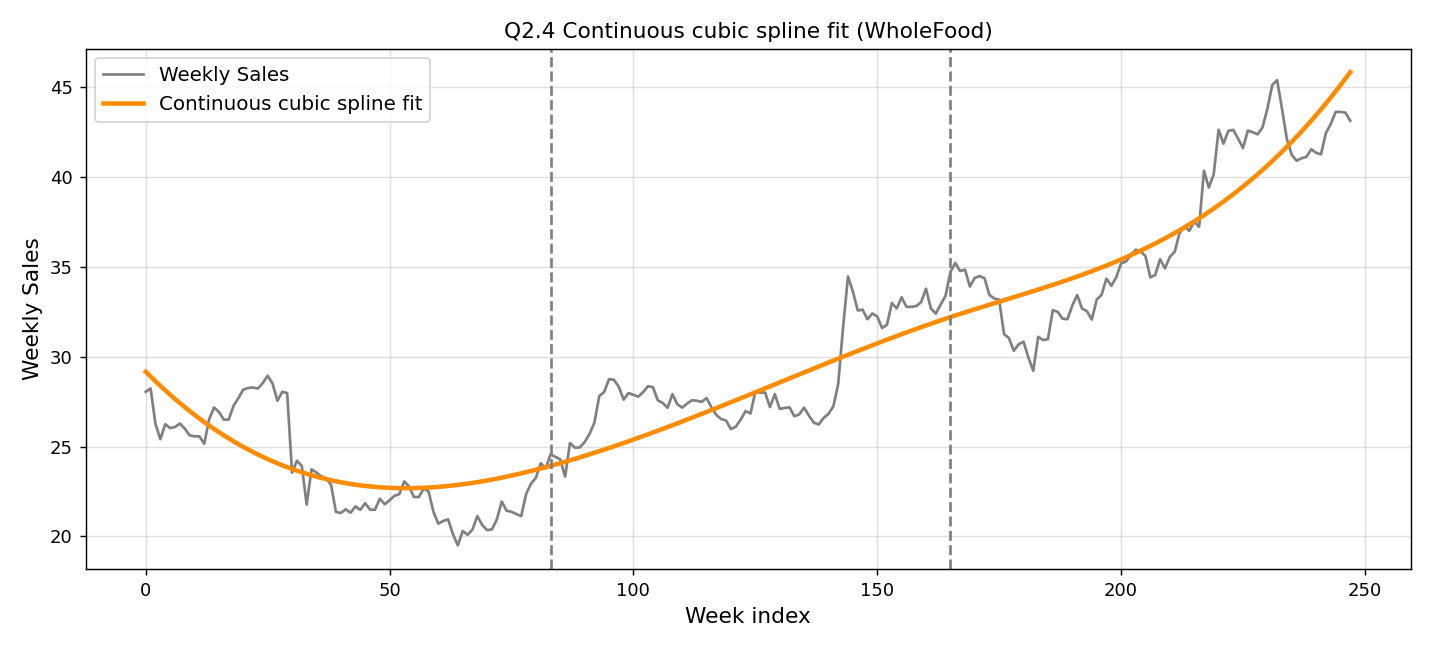
\includegraphics[width=\textwidth]{Q2_cubic_spline.png}
     \caption{Q2.4 Continuous cubic spline fit. The smooth curve flatly ignores the structural breaks at week 82 and week 165.}
     \label{fig:q2_cs}
\end{figure}

\end{homeworkProblem}

\end{document}
